\begin{titlepage}

\centering

\begin{center}
\begin{tikzpicture}[remember picture, overlay]
    % VNU logo
    \node[opacity=0.2,inner sep=0pt] at (0, 0) {
\includegraphics[width=1\textwidth]{Figures/0. General/VNU_gray.png}};
    
    % HCMUS logo
    \node[inner sep=0pt] (logo) at (-3, 0) {
\includegraphics[width=.55\textwidth]{Figures/0. General/hcmus.png}};
    
    % FIT
    \node[text width=0.5\textwidth, right=of logo] (title) {
\includegraphics[width=.6\textwidth]{Figures/0. General/fit.png}};
    
    % Red line
    \draw[line width=1mm, Tue-red] ($(logo.east) + (0.5, 1.3)$) -- ($(logo.east) + (0.5, -1.3)$);
\end{tikzpicture}
\end{center}

\vspace{3cm}
\newcommand{\HRule}{\rule{\linewidth}{0.5mm}}
\HRule \\[0.4cm]
{ 
\huge{\bfseries{\reporttitle}}\\[0.5cm]
\large{\bfseries{Topic: \reportname}}
}\\[0.4cm]
\HRule \\[0.7cm]

\textbf{\large Course: \coursename}\\[0.7cm]

\begin{minipage}[t]{0.4\textwidth}
\begin{flushleft} \large
% \emph{Students execute:}\\
% \studentname
\end{flushleft}
\end{minipage}
~
\begin{minipage}[t]{0.4\textwidth}
\begin{flushright} \large
\emph{Supervisor:} \\
\teachername
\end{flushright}
\end{minipage}\\[1cm]

\large \sffamily\groupnumber

\begin{table}[H]
    \centering
    \large
    \begin{tabu} to 0.8\linewidth {cc}
        \sffamily \textbf{Full Name} & \sffamily \textbf{Student ID}\\
        \hline
        \reportauthors
    \end{tabu}
\end{table}


% \sffamily \grouptutor

\tikz[remember picture,overlay]\node[anchor=south,inner sep=0pt] at (current page.south) {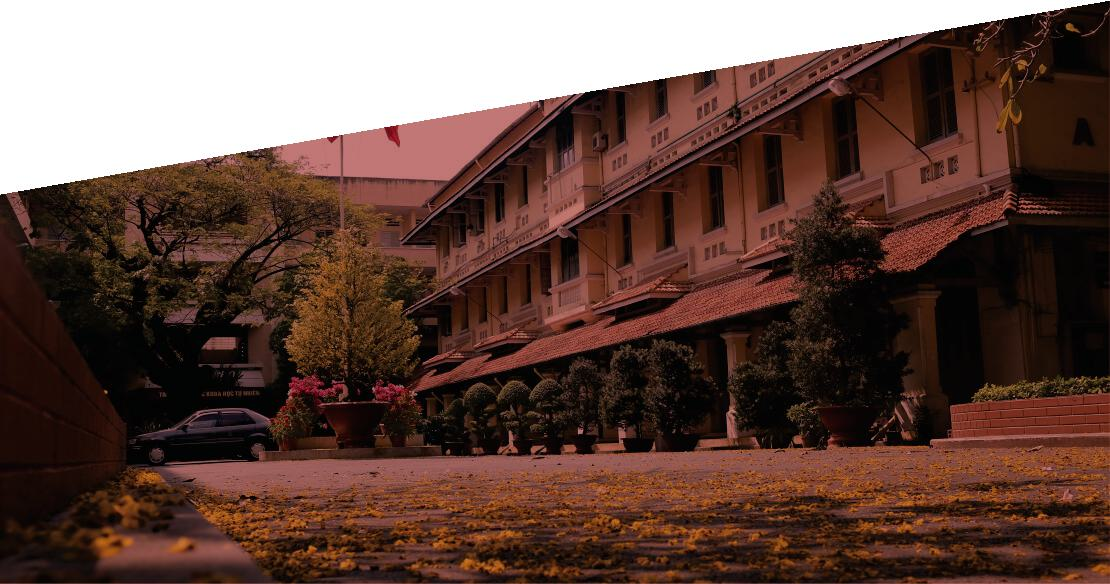
\includegraphics[width=\paperwidth]{Figures/0. General/fixed.jpeg}};

\mbox{}
\vfill
% \sffamily 
\Large \textcolor{white}{\normalfont \placeanddate} \\

\end{titlepage}








